\documentclass[main.tex]{subfiles} % Subfile-Class

%==============================================================================%
%                                   Subfile                                    %
%==============================================================================%

\begin{document}

% Template

\subsubsection{Sensorik}

\subsubsection*{Liniensensor}~\label{sec:Sensorik_Liniensensor}

Der Liniensensor aus dem Konzept aus PREN1 hat sich als sehr zuverlässig
erwiesen. Er arbeitet mit UV-Licht, das das weisse Klebeband auf den Fugen
fluoreszieren lässt, während die Fugen zwischen den Fliesen nicht
fluoreszieren. Die Beleuchtungsstärke wird im sichtbaren Spektrum ausgewertet,
sodass ausschliesslich das fluoreszierende Klebeband erfasst wird. Dies
ermöglicht einen starken Kontrast zur Umgebung.

\begin{figure}[H]
    \centering
    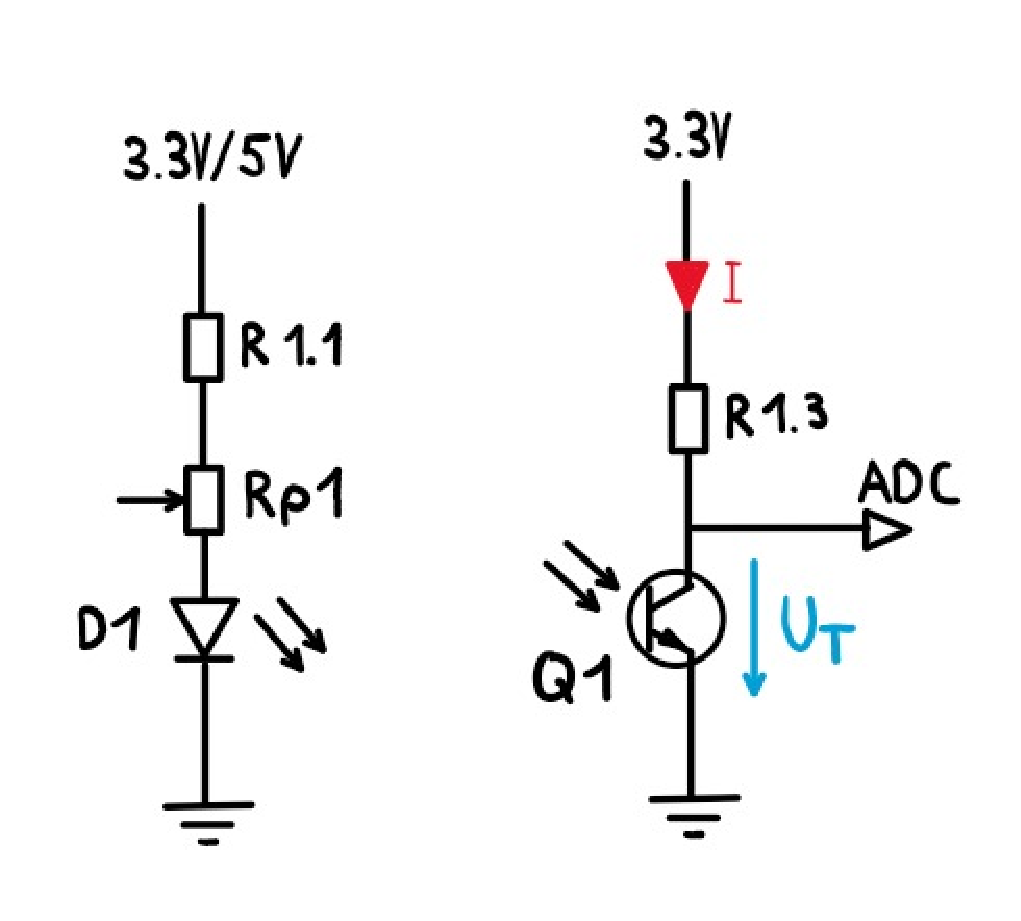
\includegraphics[width = 0.5\linewidth]{./fig_Antriebsregelung_Firmware/Schema_Messzelle_Liniensensor.pdf}
    \caption{Schema einer einzelnen Messzelle des Liniensensors}~\label{fig:Schema_Messtelle_Liniensensor}
\end{figure}

Die Dimensionierung des Sensors, welcher in
Abbildung~\ref{fig:Schema_Messtelle_Liniensensor} schematisch gezeigt ist,
basiert auf der Sättigung eines Phototransistors. Solange sich der Sensor über
einer Fliese befindet, bleibt der Phototransistor wenig leitend. Dadurch wird
der Spannungspegel hauptsächlich durch den Widerstand auf HIGH gezogen. Der
Widerstand wurde so gewählt, dass der Transistor in Sättigung gerät, sobald
sich ein Klebeband unterhalb des Sensors befindet. In diesem Fall wird der
Spannungspegel stark gegen GND gezogen, sodass eine Linie eindeutig detektiert
werden kann.

Das Gehäuse dieses Sensors, gezeigt in
Abbildung~\ref{fig:Gehaeuse_Liniensensor}, schirmt jede Messzelle einzeln stark
von der Umgebung ab. Dadurch beeinflussen sich die Messzellen weder
gegenseitig, noch werden sie durch Sonnenlicht oder andere Umwelteinflüsse
gestört. Das Gehäuse wird auf den Liniensensor aus
Abbildung~\ref{fig:LinienSensor_bottom} aufgesetzt, wodurch die Sender- und die
Empfängerdioden voneinander getrennt werden. Die Senderdioden sind in
Abbildung~\ref{fig:LinienSensor_bottom} mit einem Q, die Empfänger mit einem D
beschriftet.

\begin{figure}[H]
    \centering
    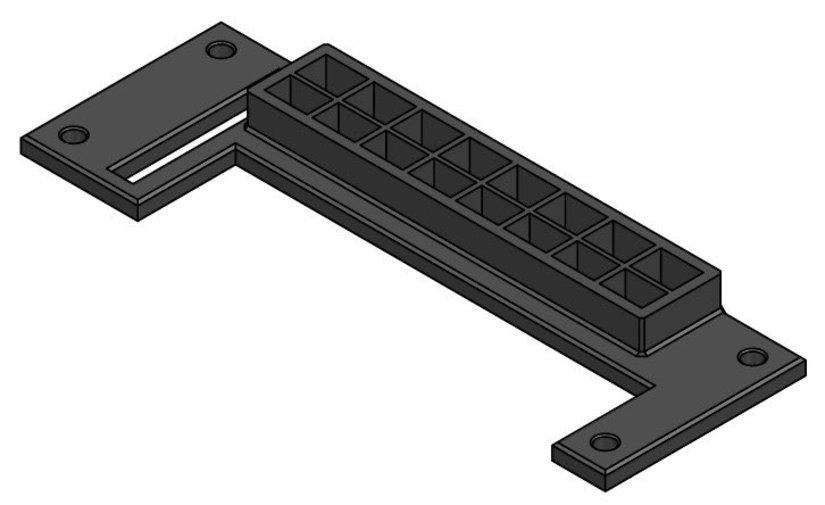
\includegraphics[width = 0.5\linewidth]{./fig_Antriebsregelung_Firmware/Gehaeuse_Isometrisch.pdf}
    \caption{Schema einer einzelnen Messzelle des Liniensensors}~\label{fig:Gehaeuse_Liniensensor}
\end{figure}

Aus Sicherheitsgründen ist die Elektronik, die diesen Sensor ansteuert, in der
Lage, die UV-LEDs ein- und auszuschalten. Diese werden nur aktiviert, wenn eine
Messung erfolgt. Falls nach zehn Messungen keine Linie gefunden wird, wird der
Messprozess abgebrochen und die UV-LEDs bleiben deaktiviert. Befindet sich der
Roboter nicht in Bewegung, werden also maximal zehn UV-Impulse ausgesendet, was
einer Zeitdauer von $\approx 100$ ms entspricht.

Die Sensordaten werden über einen Analog-Digital-Wandler ausgewertet. Nachdem
alle Zellen ausgelesen wurden, werden die Messwerte zunächst auf einen Bereich
von $0 \dots 1000$ normiert, um Bauteiltoleranzen zwischen den Zellen zu
kompensieren. Anschliessend werden die Werte \textit{gewichtet aufsummiert}.
Wie die Ermittlung der Linienposition funktioniert und wie dieser Wert in der
Regelung eingesetzt wird, ist im Anhang~\ref{apdx:LineFollowerRegler} im Detail
beschrieben.

Der Liniensensor hat zwar eine Standardkalibration, vor der Fahrt wird er
jedoch noch einmal genau kalibriert. Dazu sendet der Raspberry Hat einen
Kalibrierungsbefehl. Der MotionController führt dann 50 Messungen jeder Zelle
durch und speichert den Median dieser Messreihe separat in den
Kalibrierungswerten für jede Zelle ab. Mithilfe dieser Kalibrierungswerte wird
anschliessend die Normierung auf den Vektor von $0 \dots 1000$ berechnet.
Dieser Messvorgang muss einmal auf dem Klebeband und einmal auf dem
Fliesenboden durchgeführt werden und dauert weniger als $1 s$.

\begin{figure}[H]
    \centering
    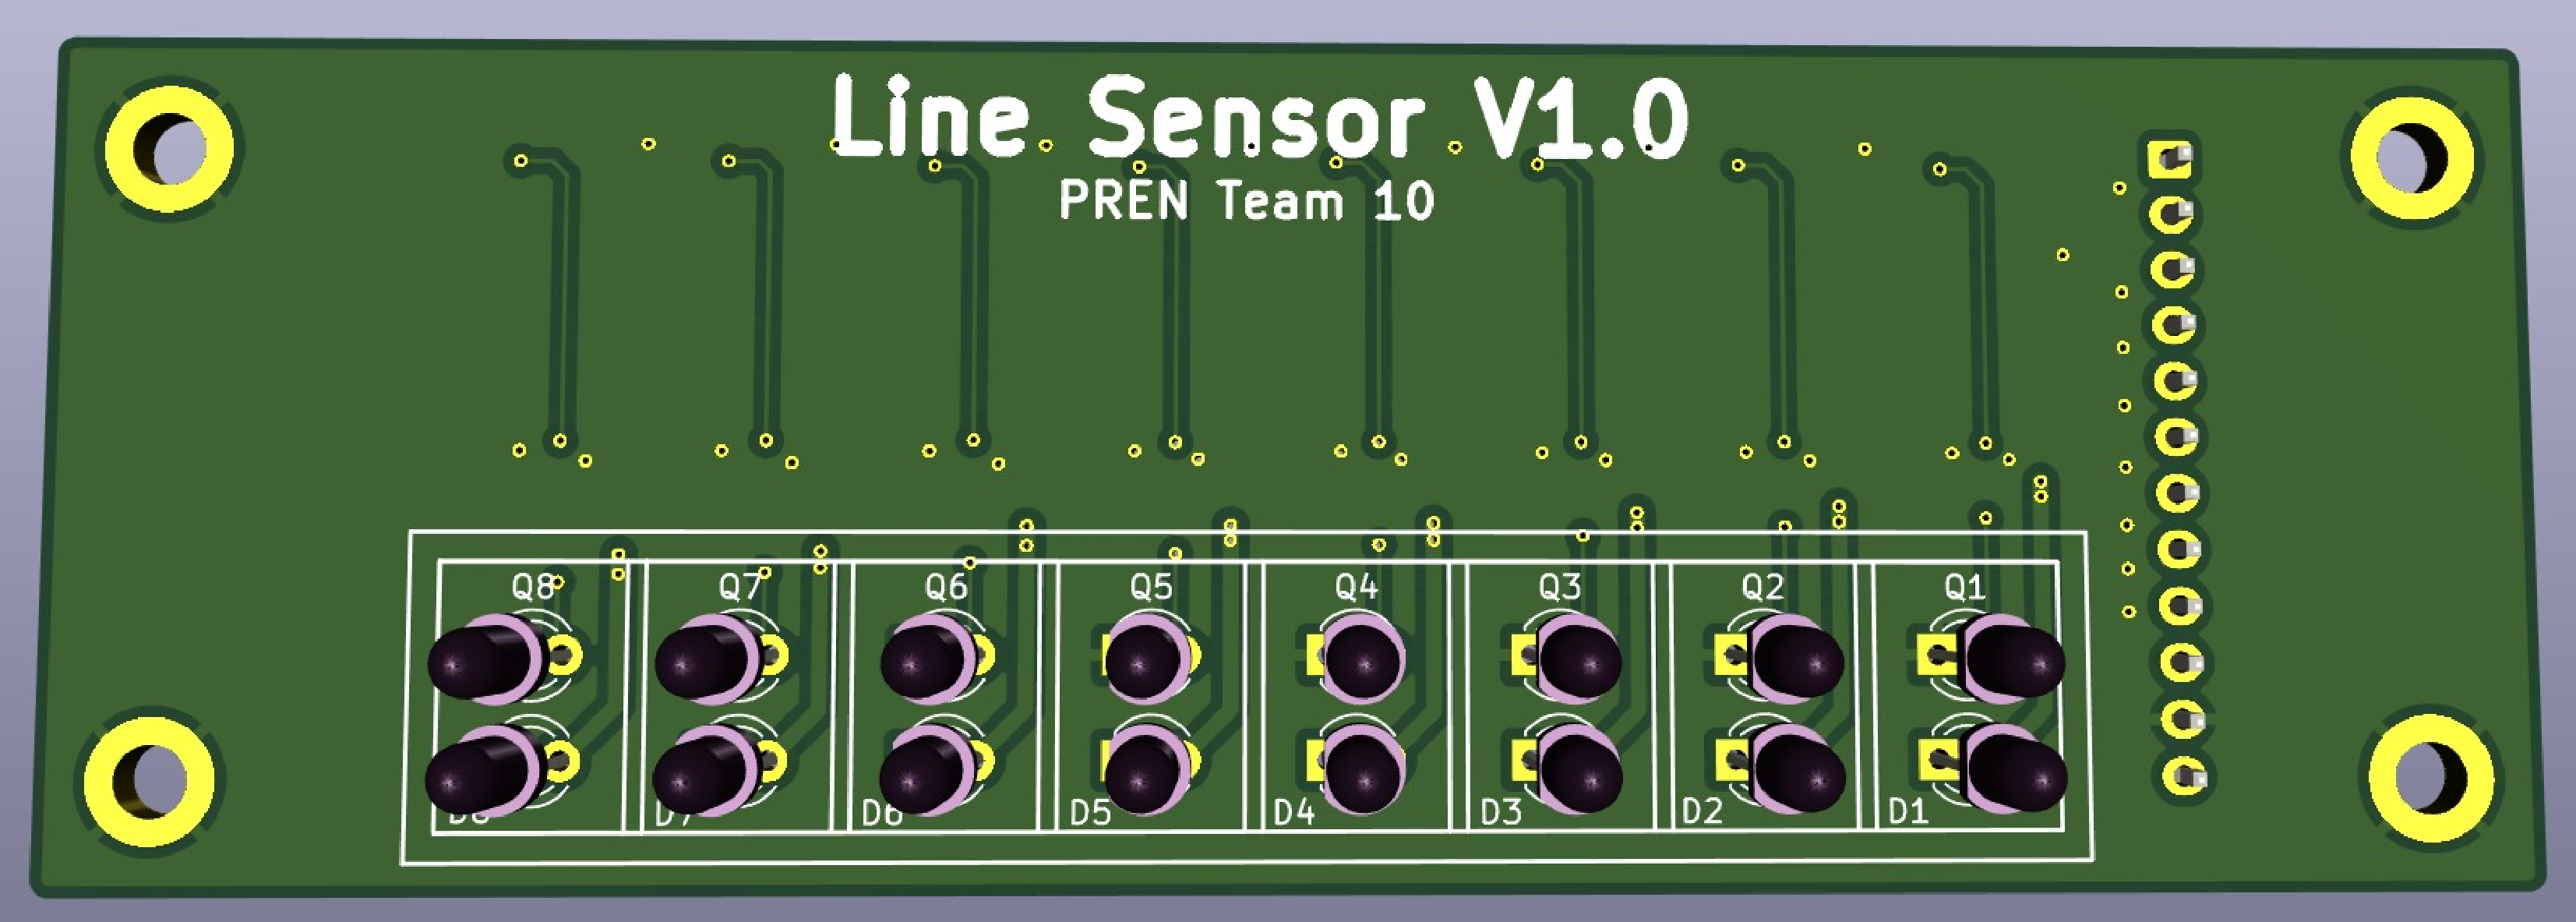
\includegraphics[width = 0.5\linewidth]{./fig_Antriebsregelung_Firmware/Liniensensor_Bottom.pdf}
    \caption{Ansicht des Liniensensors}~\label{fig:LinienSensor_bottom}
\end{figure}

Der Liniensensor ist mit einem gewissen Sensorrauschen behaftet, welches im
Anhang~\ref{apdx:Liniensensor_auswertung} nebst seiner eigentlichen Funktion
nochmals beleuchtet wird.

\subsubsection*{Streckenrückverfolgung – Distanz und Rotation}~\label{sec:Sensorik_Streckenrueckverfolgung}

Die gefahrene Strecke kann vollständig über die registrierten Schritte der
Schrittmotoren bestimmt werden. Dazu wurde die Motorbeschleunigung auf ein Mass
reduziert, das einen Schlupf der Räder verhindert. Wie die zurückgelegte
Distanz der Räder von der Firmware erfasst wird, ist im
Anhang~\ref{apdx:Distanz_Tracking} detailliert beschrieben. Die erfasste
Strecke erlaubt zudem Rückschlüsse auf die durchgeführte Rotation des
Fahrzeugs.

\subsubsection*{Erkennung von Hindernissen}~\label{sec:Sensorik_Ultraschall}

Im ursprünglichen Konzept aus PREN1 wurde die Hinderniserkennung redundant
ausgeführt: Ein Ultraschallsensor sollte die Annäherung an ein Hindernis
erkennen, während eine Laserlichtschranke den endgültigen
\textit{Greifzeitpunkt} bestimmen sollte. Aus Kostengründen wurde zunächst eine
Lösung realisiert, die ausschliesslich auf dem Ultraschallsensor basiert. Mit
verschiedenen statistischen und systemtheoretischen Methoden, die im
Anhang~\ref{apdx:FilterDimensionierungHcSr04} näher erläutert werden, lässt
sich die Position eines Hindernisses allein mit dem Ultraschallsensor sehr
genau vorhersagen.

Er erfasst gurndsätzlich nur Hindernisse, die sich näher als $500mm$ befinden.
Der Sensor hat einen Messkegel von $15°$, wodurch die gemessene Fläche nach
einer gewissen Distanz einfach zu gross wird. Dieser Sachverhalt ist in
Abbildung~\ref{fig:HcSr04_Messkegel} gezeigt.

\begin{figure}[H]
    \centering
    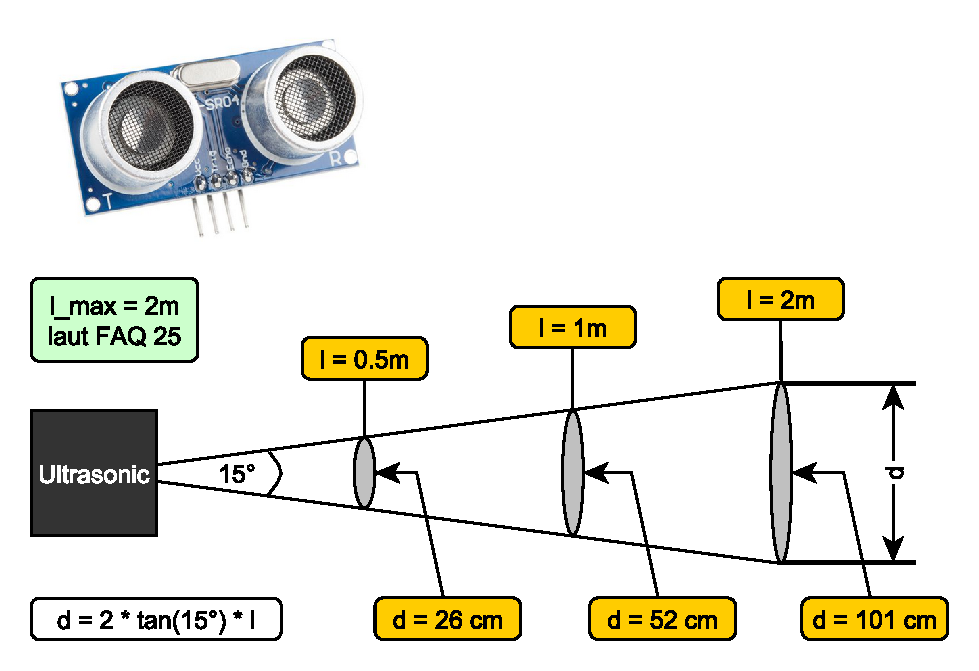
\includegraphics[width = 0.5\linewidth]{./fig_Antriebsregelung_Firmware/Auslesegenauigkeit_Ultraschall.pdf}
    \caption{Messkegel des Ultraschallsensors}~\label{fig:HcSr04_Messkegel}
\end{figure}

Ein wesentliches Problem des eingesetzten Sensors ist ebenfalls niedrige
Abfragerate für Distanzwerte. Der implementierte Filter ermöglicht jedoch eine
Vorhersage der Hindernisposition basierend auf der aktuellen
Fahrzeuggeschwindigkeit. Dadurch können auch rechnerisch ermittelte
Hindernispositionen zwischen zwei Messpunkten bestimmt werden. Nach jeder
Messung wird das Zustandsmodell korrigiert, abhängig von der Genauigkeit der
vorherigen Schätzung. Dieses Filter wird im
Anhang~\ref{apdx:Adaptiver_Tiefpass} hergeleitet und parametriert.

% TODO\ Bild Fahrzeug vor Hindernis

\subsubsection*{Pylonen LIDAR}

GABRIEL/SANDRO .. ?

\subsubsection*{Kamera}

GABRIEL

\subsubsection*{Greiferposition}

MANUEL

\end{document}
